\chapter{Code Quality and Testing}

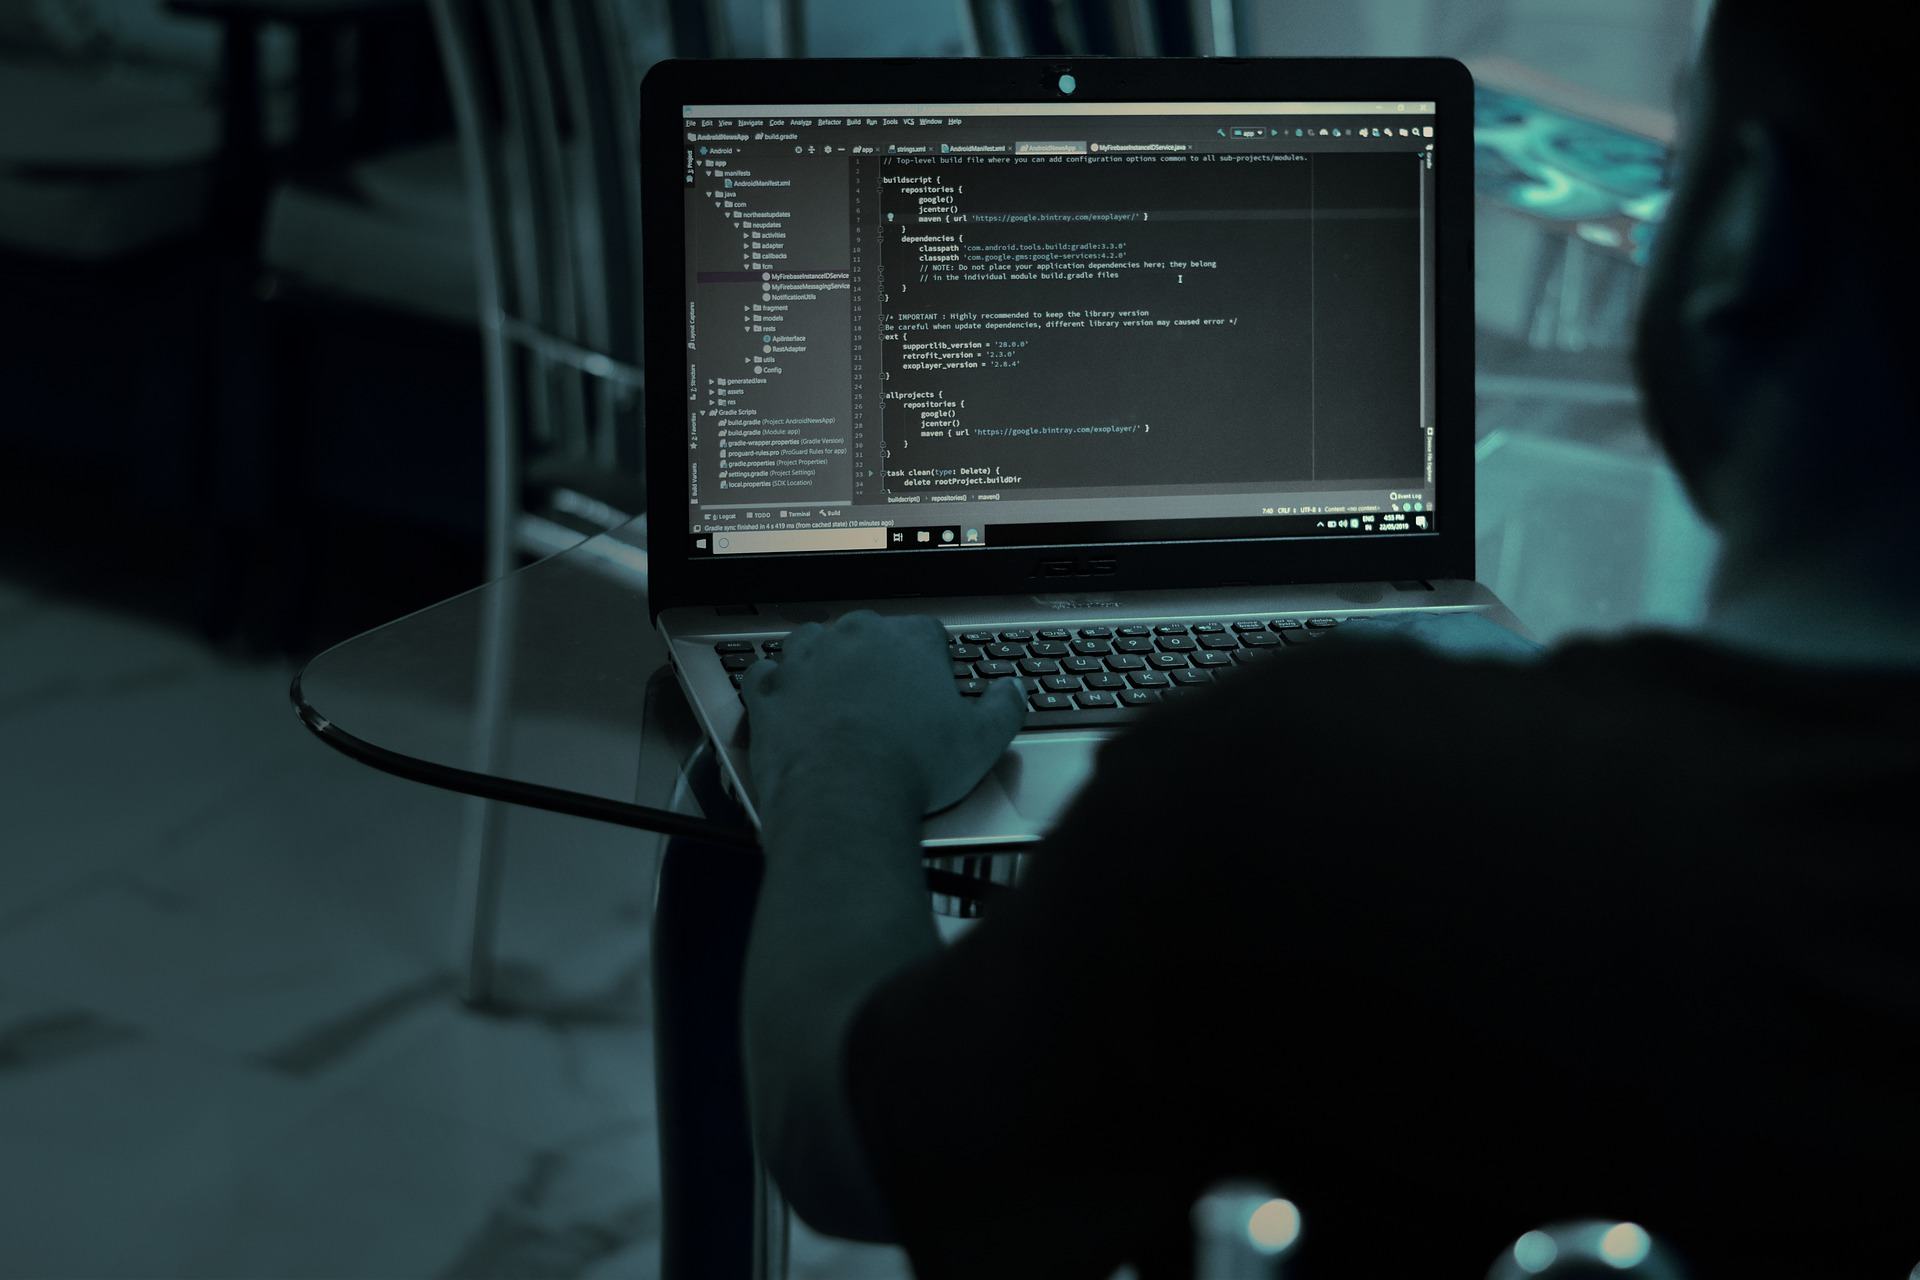
\includegraphics{26-test-quality.jpg}

\justifying
Testing our work products is vital in terms of quality and security. It is a fundamental underpinning in the ``Shift Left'' paradigm
mentioned earlier. Tesing can also be expensive in terms of money and time, making it a key target for tightening schedules by anxious project managers. Rushing through or skipping testing is a major source of defects and security issues. Many of
folks out there in the world creating software have no awareness of the concept of ``defect density'' \index{defect density},
much less how to measure it and work with their teams to reduce it.

\justifying
While it may be tempting to reduce the soak time for work products and new features in the test environment, this is generally considered a ``bad idea''. One answer to this dilemma is to reduce cycle time for testing and
improve schedule through automation and reuse of test methodologies and frameworks.

\section{Code Linting}

\markdownInput{../labs/26-test-quality/lab-9b.md}

\justifying
\begin{mybox}{\thetcbcounter: Dockerfile.fixed}
    \lstinputlisting{code/21-docker/Dockerfile.fixed}
    \label{fixeddockerfile}
\end{mybox}

\section{Unit Testing}

\justifying
Unit and functional testing is foundational in developing robust, secure code. We want to be sure that when we create new code, we are also adding
test cases to our test suite that fully cover the new classes, functions, and so on.

\justifying
Consider the following example unit test case. The purpose is to test that the function check\_docker() in the file ``src/helper\_functions.py''
returns True when called from inside a Docker container.

\begin{mybox}{\thetcbcounter: An example Unit test case}
    \lstinputlisting{code/24-python/test-unit-example.py}
\end{mybox}

\section{Automated Repository Scanning Tools}

\justifying
There are many GitHub plugins that are free for single-user/non-commercial scenarios. a cursory search of the web of the
GitHub Marketplace will turn up many of these. Let's leave some of the
tedious work to the bots, allowing us to focus on our DevSecOps journey to the cloud!

\justifying
\begin{tabular}{| p{2.3cm}| p{4.5cm} | p{8.5cm} |}
    \hline
    \textbf{Tool}& \textbf{Purpose}& \textbf{Source} \\
    \hline
    Renovate & dependency scanner & web site \\
    \hline
    lgtm & puppet-lint & Looks Good To Me \url{http://puppet-lint.com/} \\
    \hline
    metabob & AI based code review tool & website \\
    \hline
\end{tabular}

\section{Python Testing}

\justifying
Security and reliability in our lab and rapid prototyping work is just as important as it is in our work for the Production environment.
In fact, you might say it's even more important since today's rapid mock ups
can easily wind up making it into the build pipeline when folks are under a time crunch to deliver.

\justifying
There are many test frameworks out there, lots of great ideas put forth by the community. For our current
efforts, we've settled on Tox\index{Tox} as the framework of choice. It dovetails nicely with the rest of
our patterns. Tox allows us to manage requirements for virtual environments when testing, acts as a front
end to pytest and coverage modules, and much more. It is highly configurable and extensible. For example
we can test that an application is compatible with multiple versions of Python.

\justifying
Use the make test command inside the docker container to run the test suite for the project.

\justifying
An example tox.ini\index{tox.ini} file follows. Take notice of the ``deps'' section,
where Python module requirements can be specified. In our current configuration,
these are in lieu of test harness requirements specified in our
python/requirements-test.txt file.

\begin{mybox}{\thetcbcounter: An example tox.ini file}
	\lstinputlisting{code/24-python/tox.ini}
\end{mybox}

\justifying
Note that we can also include test requirements outside of our tox.ini file, as detailed in the next section.

\subsection{Python Test Requirements}

\justifying
Some requirements are strictly intended to be part of the test harness, but are not needed for the application proper. Using a separate file, such as
``src/requirements-test.txt'', makes this delineation clear to folks who are not familiar with the project.

\subsection{Test Coverage}

\justifying
As mentioned previously, we can avail ourselves of the coverage module by adding it to ``tests/test-requirements.txt'' or
the deps section of our tox.ini file. The purpose is to automatically generate a report on how much of our code
is ``covered'' by test cases in python/test.

\subsection{Linting with Tox}

Recall that we are using Tox as our main test framework. To set up Tox to do our linting work for us, we can add an environment to our envlist
called ``pylint'' and then declare it in a new stanza in tox.ini. Notice how we let ``deps'' do the work of installing the ``pylint'' dependency for
us.

\begin{mybox}{\thetcbcounter: An Example tox.ini file}
	\lstinputlisting{code/41-cicd/toxfile-pylint}
\end{mybox}

\section{Directory Structure}
\justifying
Files and folders relevant to the Test portions of our project are shown in the diagram below.

\begin{figure}[!htb]
	\centering
	\chapter{Code Quality and Testing}

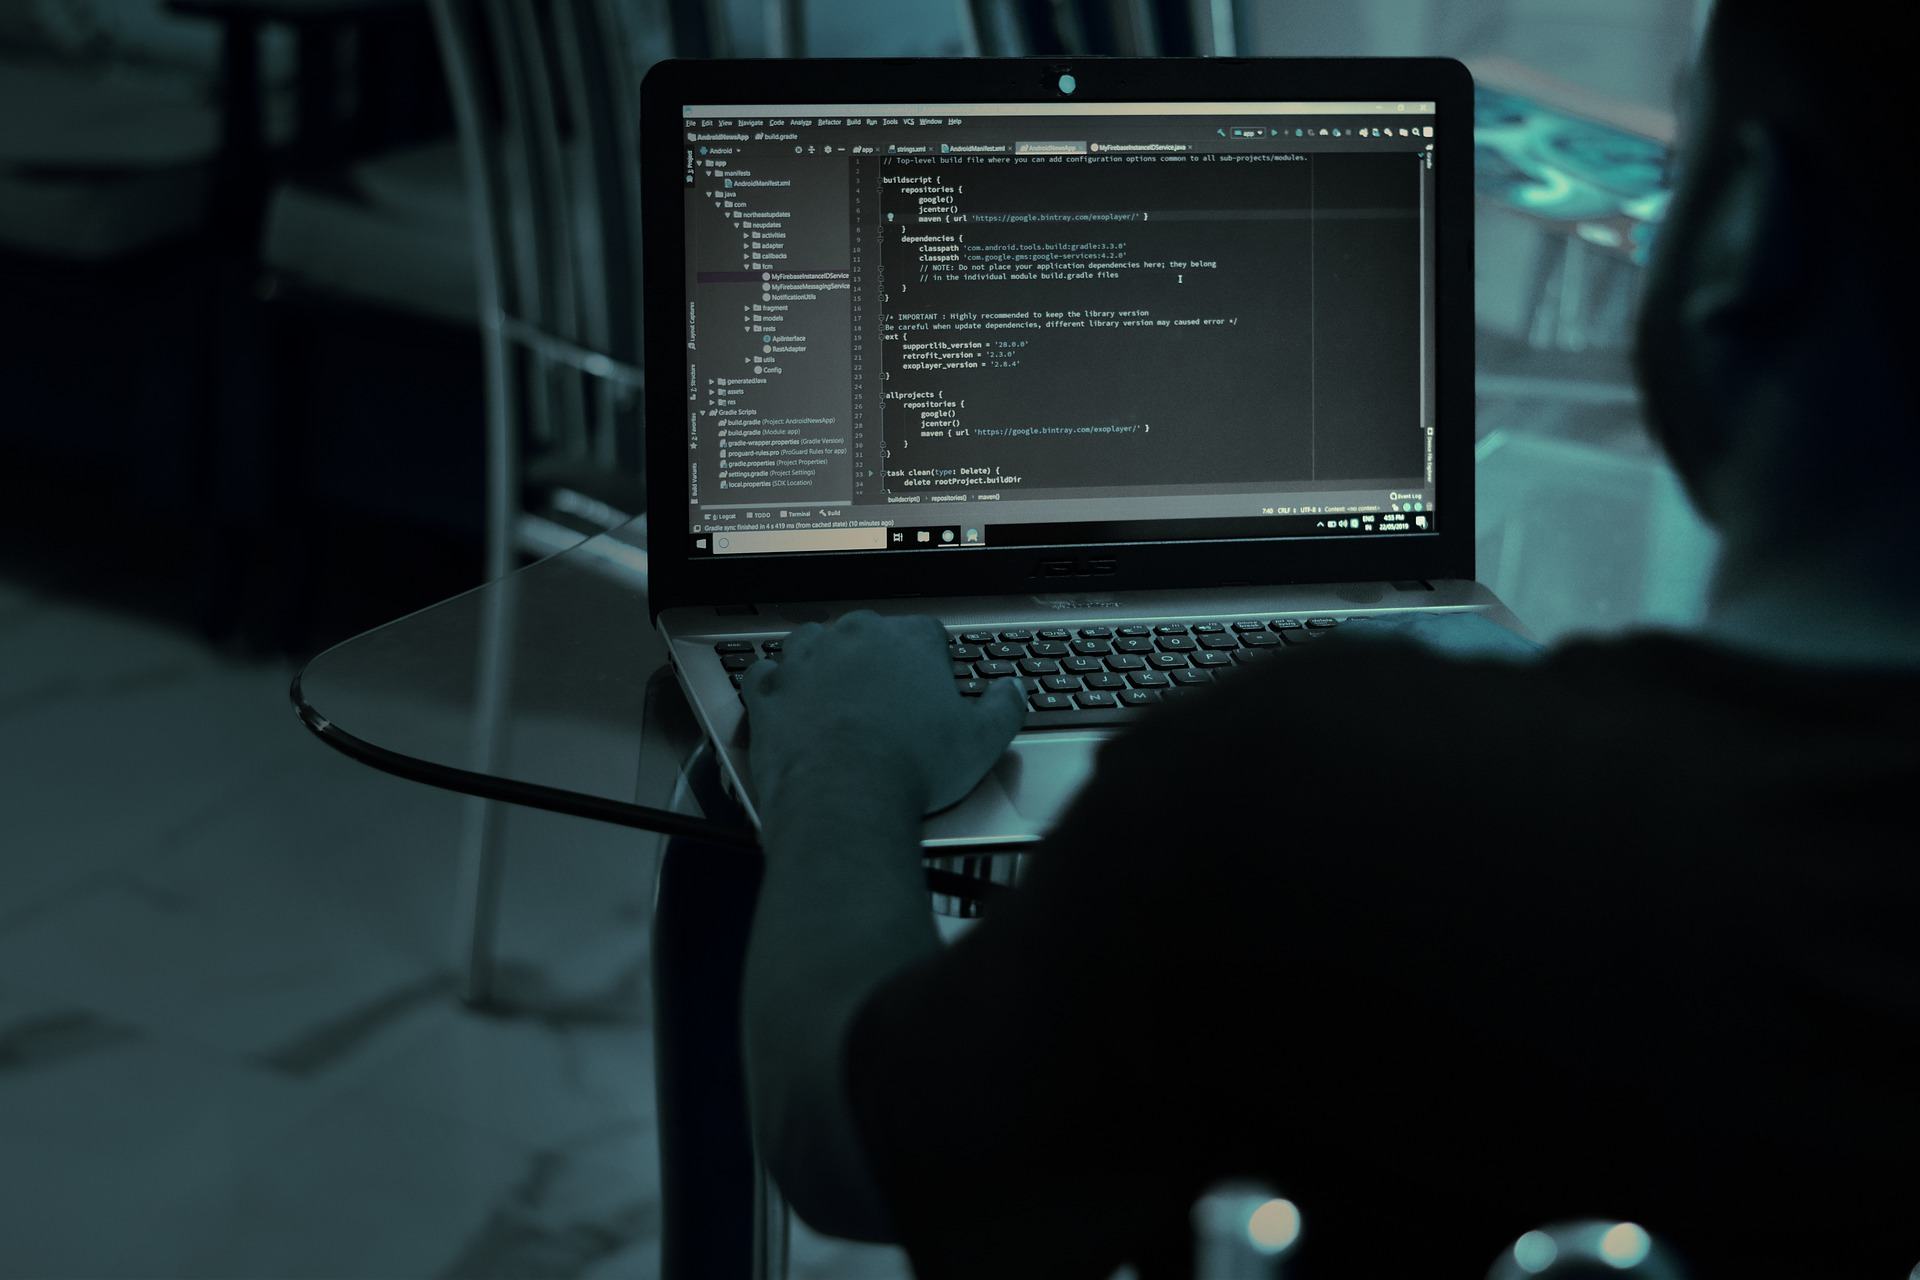
\includegraphics{26-test-quality.jpg}

	\caption{Test related files.}
	\label{testfiles}
\end{figure}
